% !TEX root = ../Thesis.tex
\acresetall
\myChapter{The mammalian lung}\label{ch:lung}
\begin{flushright}{\slshape If we're gonna move forward, this is the next logical step!} \\ \medskip
	--- Kevin Bacon as Sebastian in\defcitealias{HollowMan}{The Hollow Man}\citetalias{HollowMan} \citep{HollowMan}
\end{flushright}
\vspace{52mm}

The lung are a life-supporting, with relation to the surface one of the largest mammalian organs\graffito{The mucous surface of the intestinal tract being the largest, with a size of approximately \SI{320}{\meter\squared}~\cite{Takahashi1999}, the skin being distant third with approximately \SI{2}{\meter\squared}~\cite{Haycock1978}.}. Its function is essential for the transport of oxygen from the air we breathe into the blood and for the transport of carbon dioxide from biological processes out of the blood stream back into the atmosphere.

\section{Lung Development}
During lung development all the internal structures like the conducting airways, the blood vessel network and the gas exchange area are formed. The lung is specifically designed to provide this large gas exchange surface---in humans an area equivalent to about $\frac{3}{4}$ of a tennis court, \SI{130}{\meter\squared}~\cite{Weibel2009}---where capillary blood efficiently gets in close contact to the air inside the lung structure. This close contact is necessary for the exchange of oxygen from the inhaled air into the blood and carbon dioxide from the blood into the air to be exhaled from the body.

Mammalian lung development can be divided into five overlapping stages~\cite{Schittny2004,Schittny2007a}, as shown in \autoref{fig:lung development stages old}: Organogenesis starts with a outpouching of the foregut resulting in the appearance of the lung buds and formation of the major airways. Subsequently, the conducting and parts of the respiratory airways are formed by a successive cycle of branching and growth starting at the lung buds, which is called branching morphogenesis. Most of this process takes place during the first lung development stage, the pseudoglandular stage. In this stage the functional respiratory lung unit, the so-called acinus is formed. An acinus is defined as the complex of alveolated airways distal of a last purely conducting airway, the terminal bronchiole~\cite{Rodriguez1987}. The total of all acini forms the lung parenchyma, the area where the pulmonary gas-exchange takes place.

\begin{figure}
	\noindent\makebox[\textwidth]{%
		\centering%
		%\documentclass{article}
%\usepackage{tikz,pgfplots}
%\usepackage[graphics,tightpage,active]{preview}
%\PreviewEnvironment{tikzpicture}
%\begin{document}
%%%%%%%%%%%%%%%%%%%%%%%%%%%%%%%%%%%%%%%%%%%%%%%%%%%%%%%%%%%%%%
	\pgfplotsset{width=\linewidth,height=.5\linewidth}
	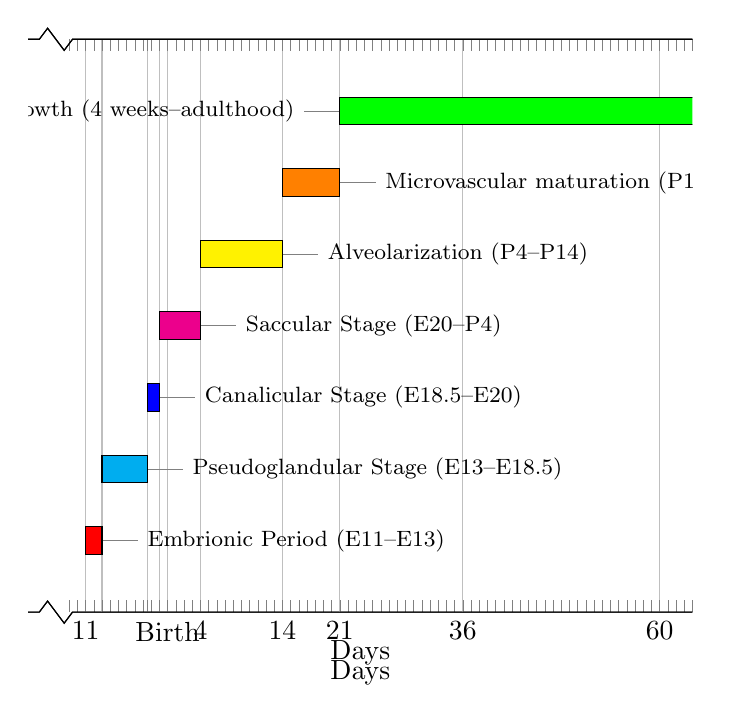
\begin{tikzpicture}
		\def\xmin{4}
		\def\xmax{85}
		\def\ymin{0}
		\def\ymax{0.4}
		\begin{axis}[xbar stacked,%
			scale only axis,%
			xmin=\xmin,%
			xmax=\xmax,%
			ymin=\ymin,%
			ymax=\ymax,%
			yticklabels={},%
			axis x discontinuity=crunch,%
			xtick={9,...,\xmax},%
			xticklabels={},
			xlabel=Days,%
			axis y line=none]
		\end{axis}
		\begin{axis}[xbar stacked,%
			scale only axis,%
			xmin=\xmin,%
			xmax=\xmax,%
			ymin=\ymin,%
			ymax=\ymax,%
			yticklabels={},%
			axis x discontinuity=crunch,%
			xtick={11,13,18.5,20,21,25,35,42,57,81},%
			xticklabels={11,,,,Birth,4,14,21,36,60},
			xmajorgrids,%
			xlabel=Days,%
			%axis x line=bottom,%
			axis y line=none]
			\def\step{0.05}
			%\node [font=\footnotesize] at (axis cs:42,0.35) {X};
			%\node [font=\footnotesize] at (axis cs:85,0.35) {X};
			%\node [font=\footnotesize] at (axis cs:63.5,0.35) {Lung Growth (4 weeks--adulthood)};
			\addplot [transparent]	coordinates {(11,0)};
			\addplot [fill=red]		coordinates {(2,1*\step)};
			\addplot [fill=cyan]		coordinates {(5.5,2*\step)};
			\addplot [fill=blue]		coordinates {(1.5,3*\step)};
			\addplot [fill=magenta]	coordinates {(5,4*\step)};
			\addplot [fill=yellow]	coordinates {(10,5*\step)};
			\addplot [fill=orange]	coordinates {(7,6*\step)};
			\addplot [fill=green]		coordinates {(\xmax-41,7*\step)};

			\tikzstyle{every pin}=[%
				%fill=white,%
				%semitransparent,%
				%draw=black,%
				%text width=10em,%
				font=\footnotesize,
				%text centered,%
				pin distance=3ex]
			\node[coordinate, pin=right:{Embrionic Period (E11--E13)}] at (axis cs:13,0.05) {};
			\node[coordinate, pin=right:{Pseudoglandular Stage (E13--E18.5)}] at (axis cs:18.5,0.1) {};
			\node[coordinate, pin=right:{Canalicular Stage (E18.5--E20)}] at (axis cs:20,0.15) {};
			\node[coordinate, pin=right:{Saccular Stage (E20--P4)}] at (axis cs:25,0.2) {};
			\node[coordinate, pin=right:{Alveolarization (P4--P14)}] at (axis cs:35,0.25) {};
			\node[coordinate, pin=right:{Microvascular maturation (P14--P21)}] at (axis cs:42,0.3) {};
			\node[coordinate, pin=left:{Lung Growth (4 weeks--adulthood)}] at (axis cs:42,0.35) {};
		\end{axis}
	\end{tikzpicture}%
%%%%%%%%%%%%%%%%%%%%%%%%%%%%%%%%%%%%%%%%%%%%%%%%%%%%%%%%%%%%%%
%\end{document}%
		}%
	\caption[Lung development stages]{Lung development stages for the rat lung according to the currently valid paradigm. The first three stages (Embryonic Period, Pseudoglandular and Canalicular Stage) take place in the approximately 21 days from the beginning of gestation to birth. E=embryonic day (days post-coitus), D=postnatal day. Figure adapted from~\cite{Schittny2007a}.}
	\label{fig:lung development stages old}
\end{figure}

The pseudoglandular stage is followed by intermediate stages, which are called canalicular and saccular. During the canalicular stage a first functional gas exchange surface---the air-blood barrier---is formed and the lung epithelium starts to differentiate. The saccular stage marks the switch from branching to septation morphogenesis.

During the alveolar stage the distal part of the bronchial tree is enlarged by the introduction of new alveoli through a formation of additional septa from already existing septa. 

After bulk alveolarization is completed, the interalveolar septa and their capillary networks are remodeled during the phase of microvascular maturation in order to optimize gas exchange. At this point lung development is considered to be finished and normal growth of the organ follows\graffito{The time point of birth differs between mammals, relative to the state of lung development. In humans, birth happens at the beginning of the alveolarization stage.}.

It was believed that lung developments comes to completion during the early postnatal period due to the reduction of a double- to a single-layered capillary network inside the alveolar septa during microvasculature maturation. After this period, only growth of the organ should follow, and no more alveolar septa are built in the lung~\cite{Burri1999,Schittny2004}. \citet{Schittny2008} were able to refine this model with an additional development stage in which the so called late alveolarization---the formation of alveolar septa until young adulthood (days 4--60 in rats)---takes place. A local duplication of the capillary network was detected as the basis of these newly forming septa.

\autoref{fig:lung development stages new} shows the refined sequence of the lung development stages. Two alveolarization phases and the phase of microvascular maturation occur simultaneously after postnatal day four until postnatal day 60. From day 60 on until adulthood only lung growth occurs, where no additional alveolar septa are introduced in the lung parenchyma.

\begin{figure}
	\noindent\makebox[\textwidth]{%
		\centering%
		% !TEX root = ../Thesis.tex
%\documentclass{article}
%\usepackage{tikz,pgfplots}
%\usepackage[graphics,tightpage,active]{preview}
%\PreviewEnvironment{tikzpicture}
%\begin{document}
%%%%%%%%%%%%%%%%%%%%%%%%%%%%%%%%%%%%%%%%%%%%%%%%%%%%%%%%%%%%%%
	\pgfplotsset{width=\linewidth,height=.5\linewidth}
	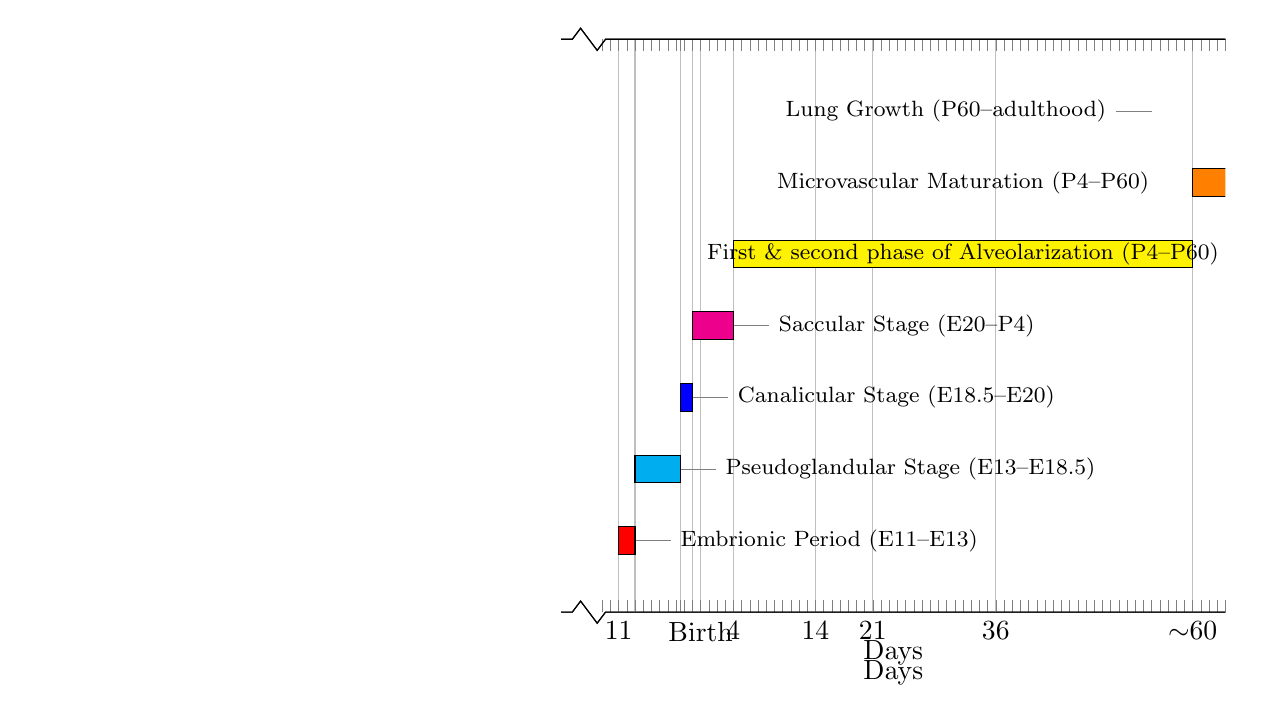
\begin{tikzpicture}
		\def\xmin{4}
		\def\xmax{85}
		\def\ymin{0}
		\def\ymax{0.4}
		\begin{axis}[xbar stacked,%
			scale only axis,%
			xmin=\xmin,%
			xmax=\xmax,%
			ymin=\ymin,%
			ymax=\ymax,%
			yticklabels={},%
			axis x discontinuity=crunch,%
			xtick={9,...,\xmax},%
			xticklabels={},
			xlabel=Days,%
			axis y line=none]
		\end{axis}
		\begin{axis}[xbar stacked,%
			scale only axis,%
			xmin=\xmin,%
			xmax=\xmax,%
			ymin=\ymin,%
			ymax=\ymax,%
			yticklabels={},%
			axis x discontinuity=crunch,%
			xtick={11,13,18.5,20,21,25,35,42,57,81},%
			xticklabels={11,,,,Birth,4,14,21,36,$\sim$60},
			xmajorgrids,%
			xlabel=Days,%
			%axis x line=bottom,%
			axis y line=none]
			%\node [font=\footnotesize] at (axis cs:25,0.25) {X};
			%\node [font=\footnotesize] at (axis cs:81,0.25) {X};
			\node [font=\footnotesize] at (axis cs:53,0.25) {First \& second phase of Alveolarization (P4--P60)};
			\node [font=\footnotesize] at (axis cs:53,0.3) {Microvascular Maturation (P4--P60)};
			\def\step{0.05}
			\addplot [transparent]	coordinates {(11,0)};
			\addplot [fill=red]		coordinates {(2,1*\step)};
			\addplot [fill=cyan]		coordinates {(5.5,2*\step)};
			\addplot [fill=blue]		coordinates {(1.5,3*\step)};
			\addplot [fill=magenta]	coordinates {(5,4*\step)};
			\addplot [fill=yellow]	coordinates {(56,5*\step)};
			\addplot [transparent]	coordinates {(-56,5.5*\step)};
			\addplot [fill=orange]	coordinates {(56,6*\step)};
			\addplot [transparent]	coordinates {(-5,5.5*\step)};
			\addplot [fill=green]		coordinates {(\xmax-75,7*\step)};
			\tikzstyle{every pin}=[%
				%fill=white,%
				%semitransparent,%
				%draw=black,%
				%text width=10em,%
				font=\footnotesize,
				%text centered,%
				pin distance=3ex]
			\node[coordinate, pin=right:{Embrionic Period (E11--E13)}] at (axis cs:13,0.05) {};
			\node[coordinate, pin=right:{Pseudoglandular Stage (E13--E18.5)}] at (axis cs:18.5,0.1) {};
			\node[coordinate, pin=right:{Canalicular Stage (E18.5--E20)}] at (axis cs:20,0.15) {};
			\node[coordinate, pin=right:{Saccular Stage (E20--P4)}] at (axis cs:25,0.2) {};
			\node[coordinate, pin=left:{Lung Growth (P60--adulthood)}] at (axis cs:76,0.35) {};
		\end{axis}
	\end{tikzpicture}%
%%%%%%%%%%%%%%%%%%%%%%%%%%%%%%%%%%%%%%%%%%%%%%%%%%%%%%%%%%%%%%
%\end{document}%
		}%
	\caption[Lung development stages]{Lung development stages with concurrently occurring Alveolarization and Microvascular Maturation stages. E=embryonic day (days post-coitus), D=postnatal day. Unpublished data from private communication with Johannes C.\ Schittny.}
	\label{fig:lung development stages new}
	\todo[inline]{Does lung growth really only start after day 60? No overlap?}
\end{figure}

\subsection{The functional units of the lung}
The airway structure of the mammalian lung is formed from dichotomous branches, starting from the trachea. The first branching generations lead into the bronchi (\autoref{subfig:lung diagram}). With increasing depth into the airway tree, the diameter of the airways is reduced, the bronchi are divided into bronchioles, leading to the terminal bronchioles which mark the end of the purely conducting airways. The start of the gas-exchange region in the lung is marked by the respiratory bronchioles, we reach the acinus and the so-called acinar airways. An acinus is---ongoing from the respiratory bronchioles---further subdivided into alveolar ducts, sacculi and alveoli (\autoref{subfig:lung units})\todo{Citation about stages needed: Use \citet{Weibel2009}?}.

\renewcommand{\imsize}{0.55\linewidth}
\begin{figure}
	\centering%
	\subfloat[]{%
		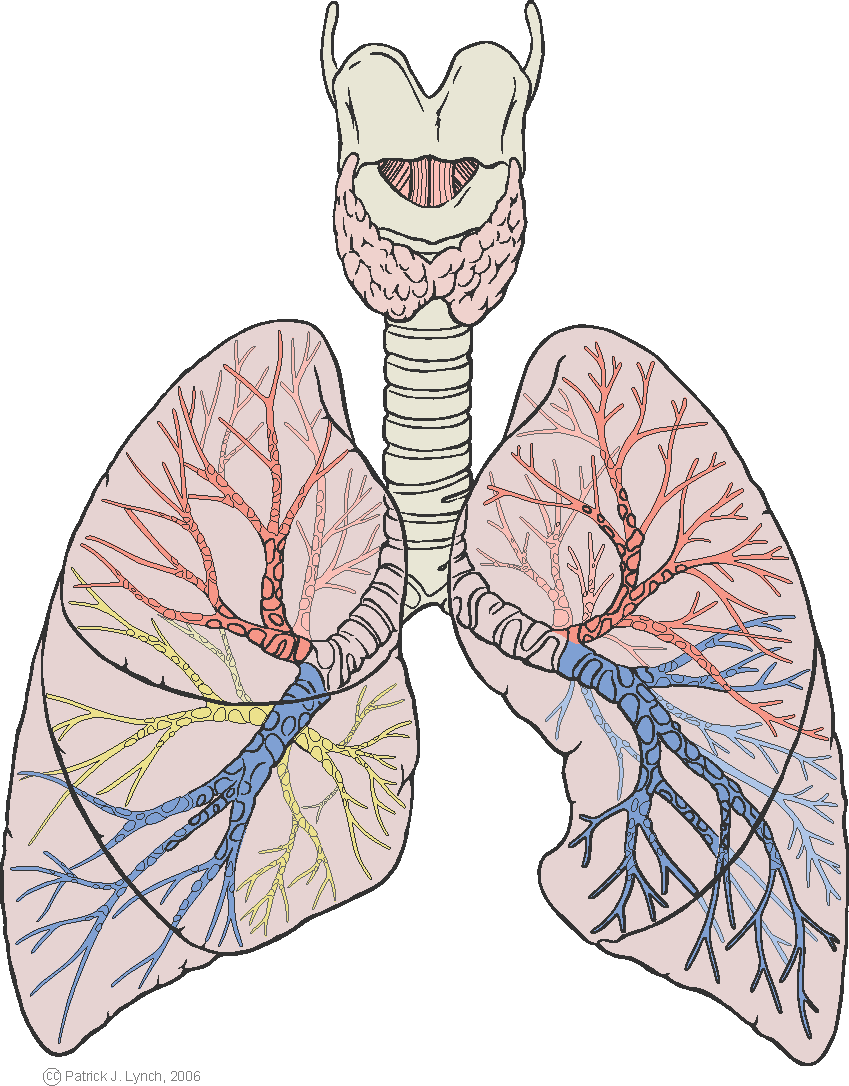
\includegraphics[width=\imsize]{img/Lungs_diagram_detailed}%
		\label{subfig:lung diagram}%
		}%
		\hfill%
	\subfloat[]{%
		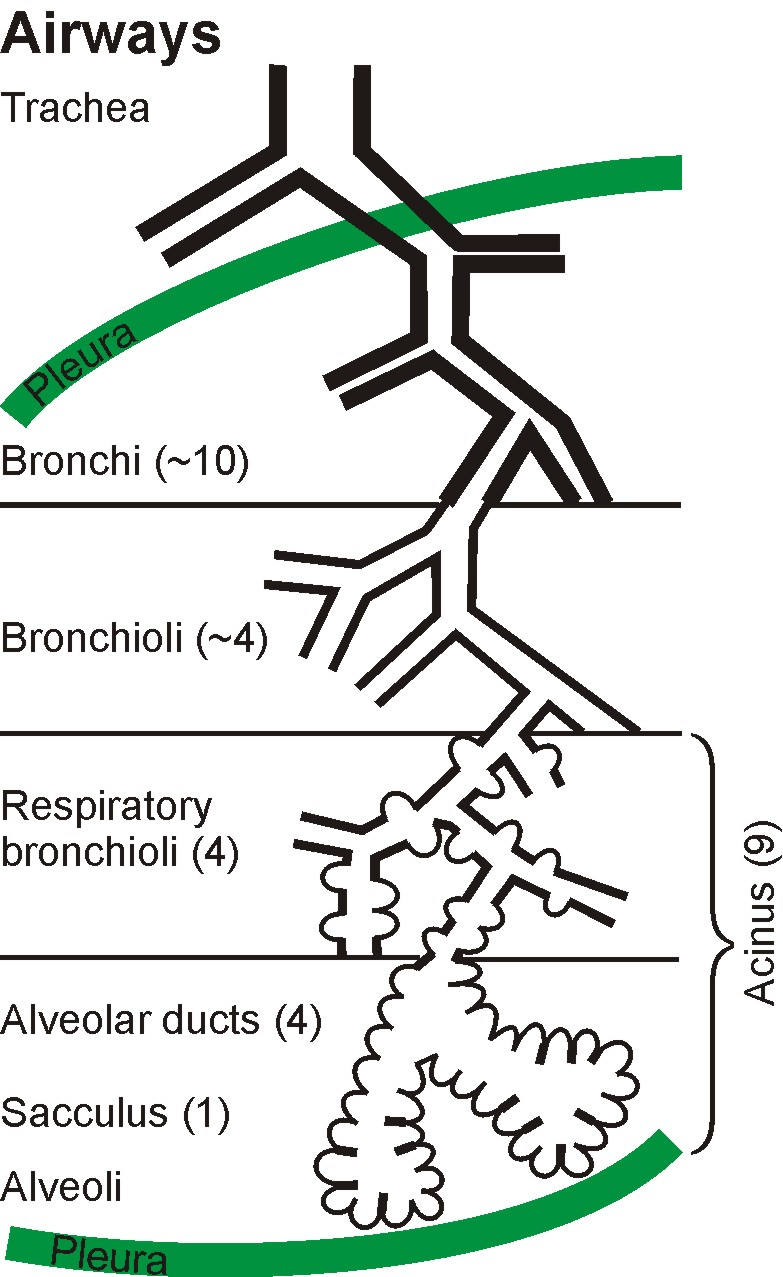
\includegraphics[height=0.7031\linewidth]{img/Lungunits}%
		\label{subfig:lung units}%
		}%
	\caption[Details of the human lung]{Details of the human lung. \subref{subfig:lung diagram}: Lung diagram of the human lung~\cite{LungDiagram}. \subref{subfig:lung units}: Airway generations in the human lung \cite{Schittny2007a}.}%
	\label{fig:lung}%
	\todo[inline]{Figure \subref{subfig:lung units} is describing the human lung. Is there a similar graph for rat or mouse?}
\end{figure}

\section{Why Tomography?}
In our group there has been an ongoing effort to analyze the parenchymal structure of the rat and mouse lung, two laboratory animals which are extensively used in respiratory research. \citet{Mund2008} challenged the model of alveolarization---the enlargement of the gas exchange surface through lifting off of new septa of the pre-existing septa~\cite{Burri1974}---and developed a working theory on late alveolarization\todo{List other notable efforts?}.

Traditionally, quantitative information and physical properties of the lung structure are obtained using stereology~\cite{Ochs2006}. Stereology refers to the mathematical methods for defining these properties of an irregular three-dimensional structure using two-dimensional planar sections obtained by physical or optical imaging techniques~\cite{Hsia2010}.

Stereology is considered to be the standard method for unbiased analysis of morphological values in the lung like three-dimensional volume or size, two-dimensional surface area, one-dimensional length and thickness of structures or \textit{global} number of alveoli. Nonetheless, certain parameters of the lung structure like the topological characteristics of the airway tree, the exact of size of \textit{single} acini and which alveolus is ventilated by which alveolar duct cannot be determined using stereological methods, but need analysis of the three-dimensional relations using tomographic data.

Additionally, the simulation of deposition of particles inside the lung based on the simulation of the airflow characteristics in the terminal airway ends is only possible with three-dimensional reconstructions of the lung tissue. For extremely small regions of the lung \citet{Woodward2005} achieved interesting results using 60 serial sections of Muscovy duck lungs with a thickness of \SI{300}{\nano\meter} each. Tremendous effort was used to reconstruct a very small volume of the lung. The volume of such a reconstruction of the terminal airways would be much too small for any of the above mentioned simulations.

Using tomographic microscopy, especially \ac{srxtm} three-dimensional data of lung samples with a volume of 1.5$\times$1.5$\times$\SI{1.5}{\milli\meter}\graffito{Even larger volumes can be acquired with this resolution, see \autoref{ch:haberthuer2010}.} with a resolution high enough to resolve the alveolar septa can be acquired in a matter of minutes~\cite{Hintermueller2010}. Since the three-dimensional data allows a fully unrestricted view into the terminal airway ends, such datasets are very well suited to answer all the above mentioned questions.

The following chapter introduces the basic concepts for computed tomography and describes the machine which was used to obtain all tomographic data for the experiments presented in this thesis.